
% Default to the notebook output style

    


% Inherit from the specified cell style.




    
\documentclass[11pt]{article}

    
    
    \usepackage[T1]{fontenc}
    % Nicer default font (+ math font) than Computer Modern for most use cases
    \usepackage{mathpazo}

    % Basic figure setup, for now with no caption control since it's done
    % automatically by Pandoc (which extracts ![](path) syntax from Markdown).
    \usepackage{graphicx}
    % We will generate all images so they have a width \maxwidth. This means
    % that they will get their normal width if they fit onto the page, but
    % are scaled down if they would overflow the margins.
    \makeatletter
    \def\maxwidth{\ifdim\Gin@nat@width>\linewidth\linewidth
    \else\Gin@nat@width\fi}
    \makeatother
    \let\Oldincludegraphics\includegraphics
    % Set max figure width to be 80% of text width, for now hardcoded.
    \renewcommand{\includegraphics}[1]{\Oldincludegraphics[width=.8\maxwidth]{#1}}
    % Ensure that by default, figures have no caption (until we provide a
    % proper Figure object with a Caption API and a way to capture that
    % in the conversion process - todo).
    \usepackage{caption}
    \DeclareCaptionLabelFormat{nolabel}{}
    \captionsetup{labelformat=nolabel}

    \usepackage{adjustbox} % Used to constrain images to a maximum size 
    \usepackage{xcolor} % Allow colors to be defined
    \usepackage{enumerate} % Needed for markdown enumerations to work
    \usepackage{geometry} % Used to adjust the document margins
    \usepackage{amsmath} % Equations
    \usepackage{amssymb} % Equations
    \usepackage{textcomp} % defines textquotesingle
    % Hack from http://tex.stackexchange.com/a/47451/13684:
    \AtBeginDocument{%
        \def\PYZsq{\textquotesingle}% Upright quotes in Pygmentized code
    }
    \usepackage{upquote} % Upright quotes for verbatim code
    \usepackage{eurosym} % defines \euro
    \usepackage[mathletters]{ucs} % Extended unicode (utf-8) support
    \usepackage[utf8x]{inputenc} % Allow utf-8 characters in the tex document
    \usepackage{fancyvrb} % verbatim replacement that allows latex
    \usepackage{grffile} % extends the file name processing of package graphics 
                         % to support a larger range 
    % The hyperref package gives us a pdf with properly built
    % internal navigation ('pdf bookmarks' for the table of contents,
    % internal cross-reference links, web links for URLs, etc.)
    \usepackage{hyperref}
    \usepackage{longtable} % longtable support required by pandoc >1.10
    \usepackage{booktabs}  % table support for pandoc > 1.12.2
    \usepackage[inline]{enumitem} % IRkernel/repr support (it uses the enumerate* environment)
    \usepackage[normalem]{ulem} % ulem is needed to support strikethroughs (\sout)
                                % normalem makes italics be italics, not underlines
    

    
    
    % Colors for the hyperref package
    \definecolor{urlcolor}{rgb}{0,.145,.698}
    \definecolor{linkcolor}{rgb}{.71,0.21,0.01}
    \definecolor{citecolor}{rgb}{.12,.54,.11}

    % ANSI colors
    \definecolor{ansi-black}{HTML}{3E424D}
    \definecolor{ansi-black-intense}{HTML}{282C36}
    \definecolor{ansi-red}{HTML}{E75C58}
    \definecolor{ansi-red-intense}{HTML}{B22B31}
    \definecolor{ansi-green}{HTML}{00A250}
    \definecolor{ansi-green-intense}{HTML}{007427}
    \definecolor{ansi-yellow}{HTML}{DDB62B}
    \definecolor{ansi-yellow-intense}{HTML}{B27D12}
    \definecolor{ansi-blue}{HTML}{208FFB}
    \definecolor{ansi-blue-intense}{HTML}{0065CA}
    \definecolor{ansi-magenta}{HTML}{D160C4}
    \definecolor{ansi-magenta-intense}{HTML}{A03196}
    \definecolor{ansi-cyan}{HTML}{60C6C8}
    \definecolor{ansi-cyan-intense}{HTML}{258F8F}
    \definecolor{ansi-white}{HTML}{C5C1B4}
    \definecolor{ansi-white-intense}{HTML}{A1A6B2}

    % commands and environments needed by pandoc snippets
    % extracted from the output of `pandoc -s`
    \providecommand{\tightlist}{%
      \setlength{\itemsep}{0pt}\setlength{\parskip}{0pt}}
    \DefineVerbatimEnvironment{Highlighting}{Verbatim}{commandchars=\\\{\}}
    % Add ',fontsize=\small' for more characters per line
    \newenvironment{Shaded}{}{}
    \newcommand{\KeywordTok}[1]{\textcolor[rgb]{0.00,0.44,0.13}{\textbf{{#1}}}}
    \newcommand{\DataTypeTok}[1]{\textcolor[rgb]{0.56,0.13,0.00}{{#1}}}
    \newcommand{\DecValTok}[1]{\textcolor[rgb]{0.25,0.63,0.44}{{#1}}}
    \newcommand{\BaseNTok}[1]{\textcolor[rgb]{0.25,0.63,0.44}{{#1}}}
    \newcommand{\FloatTok}[1]{\textcolor[rgb]{0.25,0.63,0.44}{{#1}}}
    \newcommand{\CharTok}[1]{\textcolor[rgb]{0.25,0.44,0.63}{{#1}}}
    \newcommand{\StringTok}[1]{\textcolor[rgb]{0.25,0.44,0.63}{{#1}}}
    \newcommand{\CommentTok}[1]{\textcolor[rgb]{0.38,0.63,0.69}{\textit{{#1}}}}
    \newcommand{\OtherTok}[1]{\textcolor[rgb]{0.00,0.44,0.13}{{#1}}}
    \newcommand{\AlertTok}[1]{\textcolor[rgb]{1.00,0.00,0.00}{\textbf{{#1}}}}
    \newcommand{\FunctionTok}[1]{\textcolor[rgb]{0.02,0.16,0.49}{{#1}}}
    \newcommand{\RegionMarkerTok}[1]{{#1}}
    \newcommand{\ErrorTok}[1]{\textcolor[rgb]{1.00,0.00,0.00}{\textbf{{#1}}}}
    \newcommand{\NormalTok}[1]{{#1}}
    
    % Additional commands for more recent versions of Pandoc
    \newcommand{\ConstantTok}[1]{\textcolor[rgb]{0.53,0.00,0.00}{{#1}}}
    \newcommand{\SpecialCharTok}[1]{\textcolor[rgb]{0.25,0.44,0.63}{{#1}}}
    \newcommand{\VerbatimStringTok}[1]{\textcolor[rgb]{0.25,0.44,0.63}{{#1}}}
    \newcommand{\SpecialStringTok}[1]{\textcolor[rgb]{0.73,0.40,0.53}{{#1}}}
    \newcommand{\ImportTok}[1]{{#1}}
    \newcommand{\DocumentationTok}[1]{\textcolor[rgb]{0.73,0.13,0.13}{\textit{{#1}}}}
    \newcommand{\AnnotationTok}[1]{\textcolor[rgb]{0.38,0.63,0.69}{\textbf{\textit{{#1}}}}}
    \newcommand{\CommentVarTok}[1]{\textcolor[rgb]{0.38,0.63,0.69}{\textbf{\textit{{#1}}}}}
    \newcommand{\VariableTok}[1]{\textcolor[rgb]{0.10,0.09,0.49}{{#1}}}
    \newcommand{\ControlFlowTok}[1]{\textcolor[rgb]{0.00,0.44,0.13}{\textbf{{#1}}}}
    \newcommand{\OperatorTok}[1]{\textcolor[rgb]{0.40,0.40,0.40}{{#1}}}
    \newcommand{\BuiltInTok}[1]{{#1}}
    \newcommand{\ExtensionTok}[1]{{#1}}
    \newcommand{\PreprocessorTok}[1]{\textcolor[rgb]{0.74,0.48,0.00}{{#1}}}
    \newcommand{\AttributeTok}[1]{\textcolor[rgb]{0.49,0.56,0.16}{{#1}}}
    \newcommand{\InformationTok}[1]{\textcolor[rgb]{0.38,0.63,0.69}{\textbf{\textit{{#1}}}}}
    \newcommand{\WarningTok}[1]{\textcolor[rgb]{0.38,0.63,0.69}{\textbf{\textit{{#1}}}}}
    
    
    % Define a nice break command that doesn't care if a line doesn't already
    % exist.
    \def\br{\hspace*{\fill} \\* }
    % Math Jax compatability definitions
    \def\gt{>}
    \def\lt{<}
    % Document parameters
    \title{Untitled}
    
    
    

    % Pygments definitions
    
\makeatletter
\def\PY@reset{\let\PY@it=\relax \let\PY@bf=\relax%
    \let\PY@ul=\relax \let\PY@tc=\relax%
    \let\PY@bc=\relax \let\PY@ff=\relax}
\def\PY@tok#1{\csname PY@tok@#1\endcsname}
\def\PY@toks#1+{\ifx\relax#1\empty\else%
    \PY@tok{#1}\expandafter\PY@toks\fi}
\def\PY@do#1{\PY@bc{\PY@tc{\PY@ul{%
    \PY@it{\PY@bf{\PY@ff{#1}}}}}}}
\def\PY#1#2{\PY@reset\PY@toks#1+\relax+\PY@do{#2}}

\expandafter\def\csname PY@tok@w\endcsname{\def\PY@tc##1{\textcolor[rgb]{0.73,0.73,0.73}{##1}}}
\expandafter\def\csname PY@tok@c\endcsname{\let\PY@it=\textit\def\PY@tc##1{\textcolor[rgb]{0.25,0.50,0.50}{##1}}}
\expandafter\def\csname PY@tok@cp\endcsname{\def\PY@tc##1{\textcolor[rgb]{0.74,0.48,0.00}{##1}}}
\expandafter\def\csname PY@tok@k\endcsname{\let\PY@bf=\textbf\def\PY@tc##1{\textcolor[rgb]{0.00,0.50,0.00}{##1}}}
\expandafter\def\csname PY@tok@kp\endcsname{\def\PY@tc##1{\textcolor[rgb]{0.00,0.50,0.00}{##1}}}
\expandafter\def\csname PY@tok@kt\endcsname{\def\PY@tc##1{\textcolor[rgb]{0.69,0.00,0.25}{##1}}}
\expandafter\def\csname PY@tok@o\endcsname{\def\PY@tc##1{\textcolor[rgb]{0.40,0.40,0.40}{##1}}}
\expandafter\def\csname PY@tok@ow\endcsname{\let\PY@bf=\textbf\def\PY@tc##1{\textcolor[rgb]{0.67,0.13,1.00}{##1}}}
\expandafter\def\csname PY@tok@nb\endcsname{\def\PY@tc##1{\textcolor[rgb]{0.00,0.50,0.00}{##1}}}
\expandafter\def\csname PY@tok@nf\endcsname{\def\PY@tc##1{\textcolor[rgb]{0.00,0.00,1.00}{##1}}}
\expandafter\def\csname PY@tok@nc\endcsname{\let\PY@bf=\textbf\def\PY@tc##1{\textcolor[rgb]{0.00,0.00,1.00}{##1}}}
\expandafter\def\csname PY@tok@nn\endcsname{\let\PY@bf=\textbf\def\PY@tc##1{\textcolor[rgb]{0.00,0.00,1.00}{##1}}}
\expandafter\def\csname PY@tok@ne\endcsname{\let\PY@bf=\textbf\def\PY@tc##1{\textcolor[rgb]{0.82,0.25,0.23}{##1}}}
\expandafter\def\csname PY@tok@nv\endcsname{\def\PY@tc##1{\textcolor[rgb]{0.10,0.09,0.49}{##1}}}
\expandafter\def\csname PY@tok@no\endcsname{\def\PY@tc##1{\textcolor[rgb]{0.53,0.00,0.00}{##1}}}
\expandafter\def\csname PY@tok@nl\endcsname{\def\PY@tc##1{\textcolor[rgb]{0.63,0.63,0.00}{##1}}}
\expandafter\def\csname PY@tok@ni\endcsname{\let\PY@bf=\textbf\def\PY@tc##1{\textcolor[rgb]{0.60,0.60,0.60}{##1}}}
\expandafter\def\csname PY@tok@na\endcsname{\def\PY@tc##1{\textcolor[rgb]{0.49,0.56,0.16}{##1}}}
\expandafter\def\csname PY@tok@nt\endcsname{\let\PY@bf=\textbf\def\PY@tc##1{\textcolor[rgb]{0.00,0.50,0.00}{##1}}}
\expandafter\def\csname PY@tok@nd\endcsname{\def\PY@tc##1{\textcolor[rgb]{0.67,0.13,1.00}{##1}}}
\expandafter\def\csname PY@tok@s\endcsname{\def\PY@tc##1{\textcolor[rgb]{0.73,0.13,0.13}{##1}}}
\expandafter\def\csname PY@tok@sd\endcsname{\let\PY@it=\textit\def\PY@tc##1{\textcolor[rgb]{0.73,0.13,0.13}{##1}}}
\expandafter\def\csname PY@tok@si\endcsname{\let\PY@bf=\textbf\def\PY@tc##1{\textcolor[rgb]{0.73,0.40,0.53}{##1}}}
\expandafter\def\csname PY@tok@se\endcsname{\let\PY@bf=\textbf\def\PY@tc##1{\textcolor[rgb]{0.73,0.40,0.13}{##1}}}
\expandafter\def\csname PY@tok@sr\endcsname{\def\PY@tc##1{\textcolor[rgb]{0.73,0.40,0.53}{##1}}}
\expandafter\def\csname PY@tok@ss\endcsname{\def\PY@tc##1{\textcolor[rgb]{0.10,0.09,0.49}{##1}}}
\expandafter\def\csname PY@tok@sx\endcsname{\def\PY@tc##1{\textcolor[rgb]{0.00,0.50,0.00}{##1}}}
\expandafter\def\csname PY@tok@m\endcsname{\def\PY@tc##1{\textcolor[rgb]{0.40,0.40,0.40}{##1}}}
\expandafter\def\csname PY@tok@gh\endcsname{\let\PY@bf=\textbf\def\PY@tc##1{\textcolor[rgb]{0.00,0.00,0.50}{##1}}}
\expandafter\def\csname PY@tok@gu\endcsname{\let\PY@bf=\textbf\def\PY@tc##1{\textcolor[rgb]{0.50,0.00,0.50}{##1}}}
\expandafter\def\csname PY@tok@gd\endcsname{\def\PY@tc##1{\textcolor[rgb]{0.63,0.00,0.00}{##1}}}
\expandafter\def\csname PY@tok@gi\endcsname{\def\PY@tc##1{\textcolor[rgb]{0.00,0.63,0.00}{##1}}}
\expandafter\def\csname PY@tok@gr\endcsname{\def\PY@tc##1{\textcolor[rgb]{1.00,0.00,0.00}{##1}}}
\expandafter\def\csname PY@tok@ge\endcsname{\let\PY@it=\textit}
\expandafter\def\csname PY@tok@gs\endcsname{\let\PY@bf=\textbf}
\expandafter\def\csname PY@tok@gp\endcsname{\let\PY@bf=\textbf\def\PY@tc##1{\textcolor[rgb]{0.00,0.00,0.50}{##1}}}
\expandafter\def\csname PY@tok@go\endcsname{\def\PY@tc##1{\textcolor[rgb]{0.53,0.53,0.53}{##1}}}
\expandafter\def\csname PY@tok@gt\endcsname{\def\PY@tc##1{\textcolor[rgb]{0.00,0.27,0.87}{##1}}}
\expandafter\def\csname PY@tok@err\endcsname{\def\PY@bc##1{\setlength{\fboxsep}{0pt}\fcolorbox[rgb]{1.00,0.00,0.00}{1,1,1}{\strut ##1}}}
\expandafter\def\csname PY@tok@kc\endcsname{\let\PY@bf=\textbf\def\PY@tc##1{\textcolor[rgb]{0.00,0.50,0.00}{##1}}}
\expandafter\def\csname PY@tok@kd\endcsname{\let\PY@bf=\textbf\def\PY@tc##1{\textcolor[rgb]{0.00,0.50,0.00}{##1}}}
\expandafter\def\csname PY@tok@kn\endcsname{\let\PY@bf=\textbf\def\PY@tc##1{\textcolor[rgb]{0.00,0.50,0.00}{##1}}}
\expandafter\def\csname PY@tok@kr\endcsname{\let\PY@bf=\textbf\def\PY@tc##1{\textcolor[rgb]{0.00,0.50,0.00}{##1}}}
\expandafter\def\csname PY@tok@bp\endcsname{\def\PY@tc##1{\textcolor[rgb]{0.00,0.50,0.00}{##1}}}
\expandafter\def\csname PY@tok@fm\endcsname{\def\PY@tc##1{\textcolor[rgb]{0.00,0.00,1.00}{##1}}}
\expandafter\def\csname PY@tok@vc\endcsname{\def\PY@tc##1{\textcolor[rgb]{0.10,0.09,0.49}{##1}}}
\expandafter\def\csname PY@tok@vg\endcsname{\def\PY@tc##1{\textcolor[rgb]{0.10,0.09,0.49}{##1}}}
\expandafter\def\csname PY@tok@vi\endcsname{\def\PY@tc##1{\textcolor[rgb]{0.10,0.09,0.49}{##1}}}
\expandafter\def\csname PY@tok@vm\endcsname{\def\PY@tc##1{\textcolor[rgb]{0.10,0.09,0.49}{##1}}}
\expandafter\def\csname PY@tok@sa\endcsname{\def\PY@tc##1{\textcolor[rgb]{0.73,0.13,0.13}{##1}}}
\expandafter\def\csname PY@tok@sb\endcsname{\def\PY@tc##1{\textcolor[rgb]{0.73,0.13,0.13}{##1}}}
\expandafter\def\csname PY@tok@sc\endcsname{\def\PY@tc##1{\textcolor[rgb]{0.73,0.13,0.13}{##1}}}
\expandafter\def\csname PY@tok@dl\endcsname{\def\PY@tc##1{\textcolor[rgb]{0.73,0.13,0.13}{##1}}}
\expandafter\def\csname PY@tok@s2\endcsname{\def\PY@tc##1{\textcolor[rgb]{0.73,0.13,0.13}{##1}}}
\expandafter\def\csname PY@tok@sh\endcsname{\def\PY@tc##1{\textcolor[rgb]{0.73,0.13,0.13}{##1}}}
\expandafter\def\csname PY@tok@s1\endcsname{\def\PY@tc##1{\textcolor[rgb]{0.73,0.13,0.13}{##1}}}
\expandafter\def\csname PY@tok@mb\endcsname{\def\PY@tc##1{\textcolor[rgb]{0.40,0.40,0.40}{##1}}}
\expandafter\def\csname PY@tok@mf\endcsname{\def\PY@tc##1{\textcolor[rgb]{0.40,0.40,0.40}{##1}}}
\expandafter\def\csname PY@tok@mh\endcsname{\def\PY@tc##1{\textcolor[rgb]{0.40,0.40,0.40}{##1}}}
\expandafter\def\csname PY@tok@mi\endcsname{\def\PY@tc##1{\textcolor[rgb]{0.40,0.40,0.40}{##1}}}
\expandafter\def\csname PY@tok@il\endcsname{\def\PY@tc##1{\textcolor[rgb]{0.40,0.40,0.40}{##1}}}
\expandafter\def\csname PY@tok@mo\endcsname{\def\PY@tc##1{\textcolor[rgb]{0.40,0.40,0.40}{##1}}}
\expandafter\def\csname PY@tok@ch\endcsname{\let\PY@it=\textit\def\PY@tc##1{\textcolor[rgb]{0.25,0.50,0.50}{##1}}}
\expandafter\def\csname PY@tok@cm\endcsname{\let\PY@it=\textit\def\PY@tc##1{\textcolor[rgb]{0.25,0.50,0.50}{##1}}}
\expandafter\def\csname PY@tok@cpf\endcsname{\let\PY@it=\textit\def\PY@tc##1{\textcolor[rgb]{0.25,0.50,0.50}{##1}}}
\expandafter\def\csname PY@tok@c1\endcsname{\let\PY@it=\textit\def\PY@tc##1{\textcolor[rgb]{0.25,0.50,0.50}{##1}}}
\expandafter\def\csname PY@tok@cs\endcsname{\let\PY@it=\textit\def\PY@tc##1{\textcolor[rgb]{0.25,0.50,0.50}{##1}}}

\def\PYZbs{\char`\\}
\def\PYZus{\char`\_}
\def\PYZob{\char`\{}
\def\PYZcb{\char`\}}
\def\PYZca{\char`\^}
\def\PYZam{\char`\&}
\def\PYZlt{\char`\<}
\def\PYZgt{\char`\>}
\def\PYZsh{\char`\#}
\def\PYZpc{\char`\%}
\def\PYZdl{\char`\$}
\def\PYZhy{\char`\-}
\def\PYZsq{\char`\'}
\def\PYZdq{\char`\"}
\def\PYZti{\char`\~}
% for compatibility with earlier versions
\def\PYZat{@}
\def\PYZlb{[}
\def\PYZrb{]}
\makeatother


    % Exact colors from NB
    \definecolor{incolor}{rgb}{0.0, 0.0, 0.5}
    \definecolor{outcolor}{rgb}{0.545, 0.0, 0.0}



    
    % Prevent overflowing lines due to hard-to-break entities
    \sloppy 
    % Setup hyperref package
    \hypersetup{
      breaklinks=true,  % so long urls are correctly broken across lines
      colorlinks=true,
      urlcolor=urlcolor,
      linkcolor=linkcolor,
      citecolor=citecolor,
      }
    % Slightly bigger margins than the latex defaults
    
    \geometry{verbose,tmargin=1in,bmargin=1in,lmargin=1in,rmargin=1in}
    
    

    \begin{document}
    
    
    \maketitle
    
    

    
    \section{蹦床游戏 +
墙面双拼-儿童版-产品设计案}\label{ux8e66ux5e8aux6e38ux620f-ux5899ux9762ux53ccux62fc-ux513fux7ae5ux7248-ux4ea7ux54c1ux8bbeux8ba1ux6848}

    \begin{quote}
版本: 1.1.20171221\\
编辑者: 王泽光
\end{quote}

    \subsection{修改内容}\label{ux4feeux6539ux5185ux5bb9}

    \begin{itemize}
\tightlist
\item
  增加了3个游戏内容
\item
  修改了之前4个游戏内容中遗留的一些设计问题
\item
  放弃修改3个游戏内容,保留备案
\item
  新增了设计关键点中有关安全性方面的内容
\item
  增加了文档目录(在PDF格式中锚点的跳转有问题)
\item
  调整了一些目录结构,标题文字,以及一些排版样式问题
\end{itemize}

    \subsection{设计关键点}\label{ux8bbeux8ba1ux5173ux952eux70b9}

    \begin{itemize}
\tightlist
\item
  产品面向的用户为儿童 \textbf{10} 岁以下
\item
  产品承载的人数不能太少(最好是没有硬性要求)
\item
  游戏要可随时进出,满足开放式运营,无人化运营
\item
  游戏内容设计,避免强迫用户频繁(\textless{}2秒)的在两个画面交替观察
\item
  在 \_\_240*180\_\_ 的蹦床上 \textbf{\textgreater{}3}
  人的娱乐环境,将会大大降低游戏体验, \textbf{\textgreater{}6} 人,
  \textbf{kinext} 将会无法识别多余的玩家
\item
  游戏内容的设计重点是 \textbf{简洁的趣味性}
  ,以弥补游戏玩法不足而产生的枯燥感
\item
  每个玩家的有效识别在画面中都要有 \textbf{反馈}
  ,特别是在人数较多的情况下也要有所表现.
\item
  所有游戏内容的设计都必须能够符合统一的游戏模式.
\item
  所有数值都要做成可配置的形式(不要写死)
\item
  产品可以离线运行.
\item
  联网后游戏可以 \textbf{在线更新}
  .更新后只需重新启动游戏,无需其他额外的操作.
\item
  产品为 \textbf{系列产品} ,游戏内容不能设计的过于复杂.
\item
  多人混乱游戏模式,不好设计需要让玩家根据某个短暂时机做出相应的行为
\item
  蹦床上不好设计让玩家根据某个短暂时机做出跳跃响应的行为
\item
  多人混乱游戏模式,不好精确控制某个角色.
\item
  蹦床上不好设计让玩家边跳边做手势的设计(尤其是不限制人数的产品)
\item
  双拼产品在设计和实现上有一定难度和内容开发成本,可能要考虑另外的商业模式(区别于原有系列游戏的商业模式)比如软件收费.
\item
  安全问题:

  \begin{itemize}
  \tightlist
  \item
    当投影机安装过低时,会引发安全问题,游戏内跳跃值会鼓励玩家跳跃,放大安全问题
  \item
    所以要将投影仪安装在较高的位置 \textbf{\textgreater{}300cm}
  \item
    地面和蹦床上,因人为导致的震动\晃动,不能传递到投影仪的固定位置
  \item
    避免设计需要玩家前后跳跃的玩法,有可能玩家注意力在墙面,在前后跳跃时从蹦床后面摔下来.
  \end{itemize}
\end{itemize}

    \subsection{硬件安装}\label{ux786cux4ef6ux5b89ux88c5}

    

    \begin{figure}
\centering
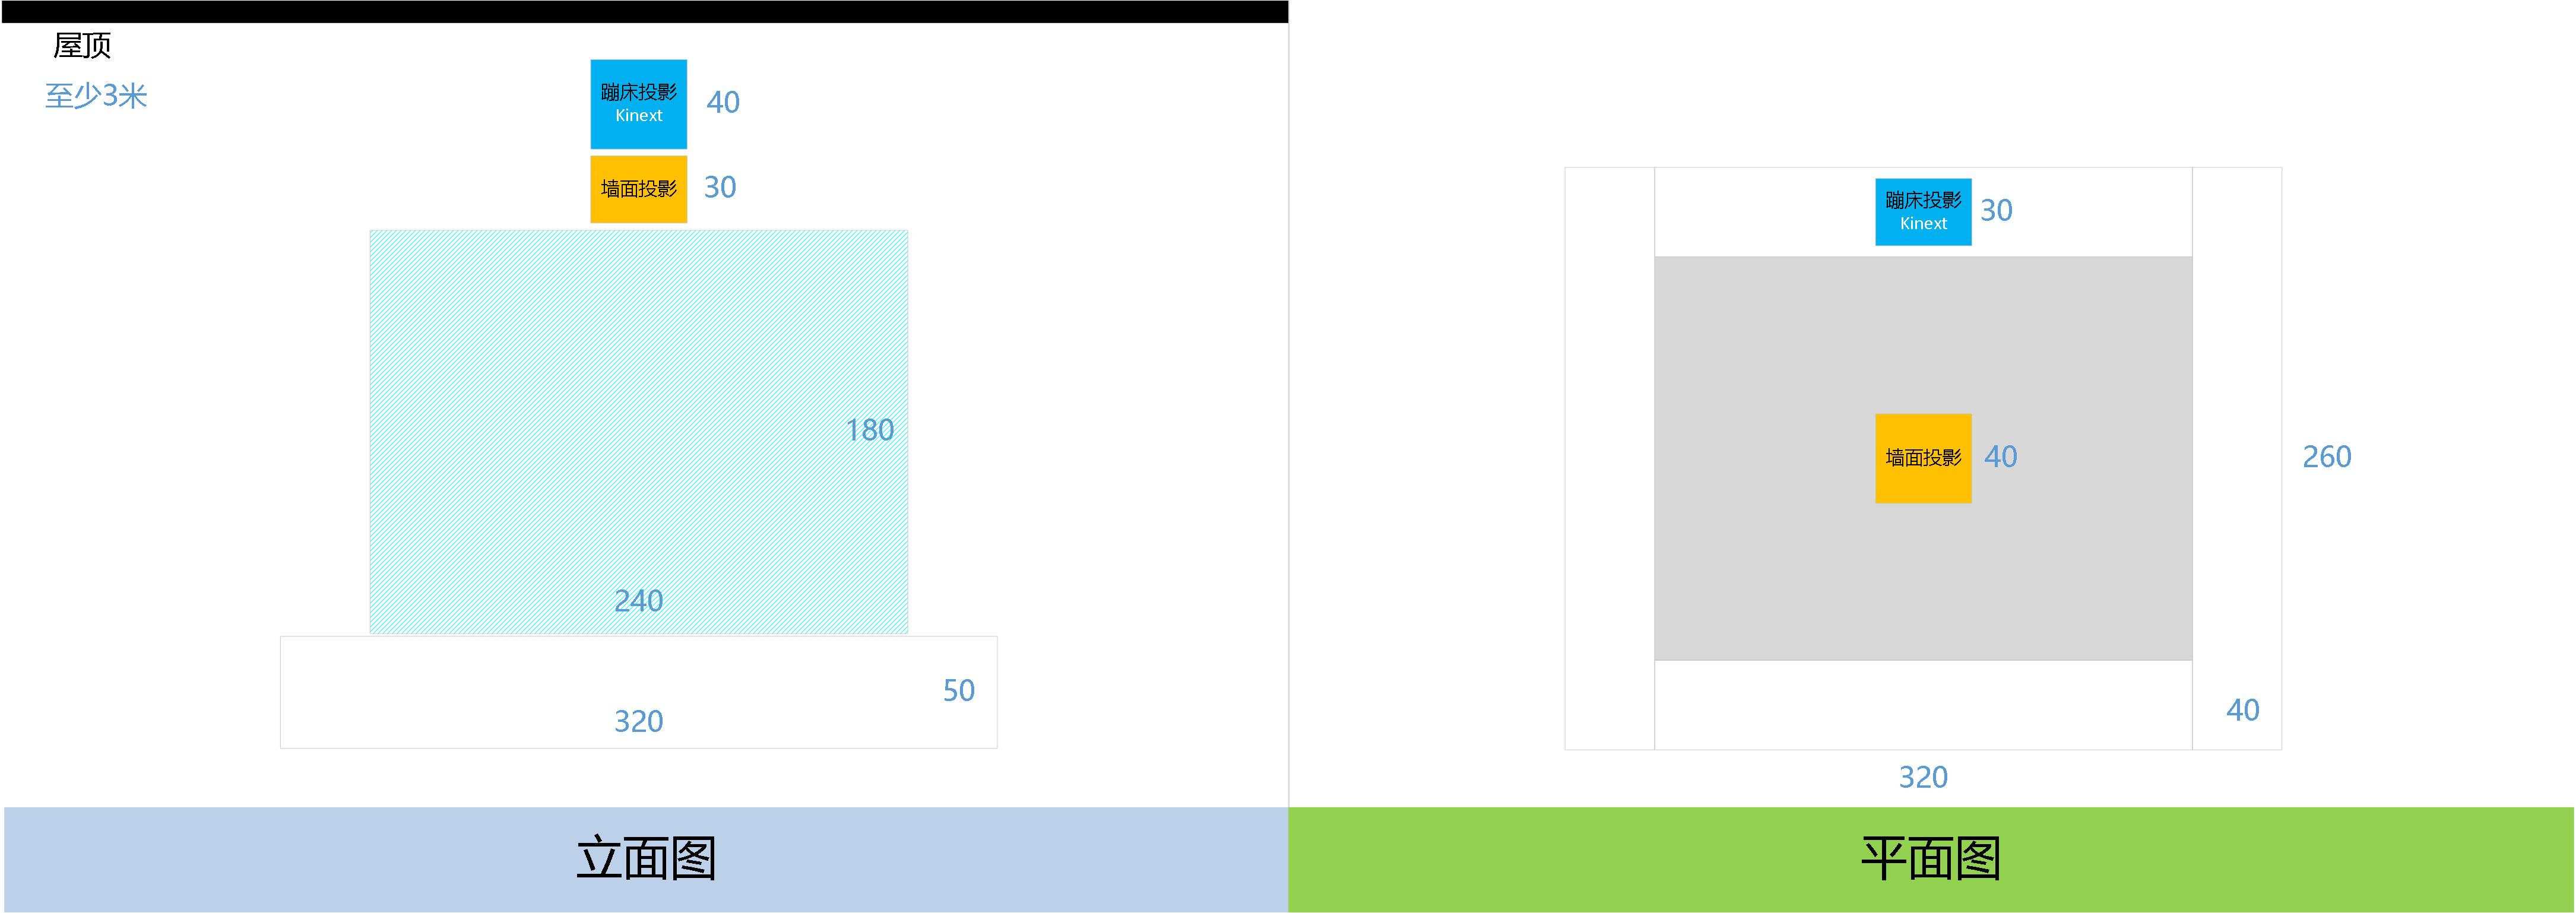
\includegraphics{111.jpg}
\caption{}
\end{figure}

    \begin{itemize}
\tightlist
\item
  展厅环境和现有一体机尺寸

  \begin{itemize}
  \tightlist
  \item
    展厅顶棚高度: \textbf{300cm}
  \item
    一体机机身深度: \textbf{40cm}
  \end{itemize}
\item
  蹦床

  \begin{itemize}
  \tightlist
  \item
    蹦床床面尺寸为: \_\_240cm*180cm\_\_ ,蹦床高度为 \textbf{50cm}
    ,软垫宽度为 \textbf{40cm}
  \item
    蹦床较宽的一面靠近墙面安放(如果时正方形蹦床则任意边靠近墙面)
  \end{itemize}
\item
  蹦床投影一体机

  \begin{itemize}
  \tightlist
  \item
    蹦床投影画面尺寸: \_\_240cm*180cm\_\_ ,宽高比为: \textbf{4:3(0.75)}
  \item
    蹦床投影画面的一体机安装在墙面投影画面的上方,靠近墙面(阴影不会遮挡画面)
  \item
    蹦床画面一体机 \textbf{包含kinext} ,用于识别玩家
  \end{itemize}
\item
  墙面投影一体机

  \begin{itemize}
  \tightlist
  \item
    墙面投影画面尺寸: \_\_240cm*180cm\_\_ ,宽高比为: \textbf{4:3(0.75)}
  \item
    墙面一体机 \textbf{不加装kinext}
  \item
    墙面一体机距离墙面的距离为: \textbf{260cm} (一体机挂架点)
  \item
    墙面投影仪挂在蹦床距离画面较远的一侧,略低于蹦床投影一体机,保证画面不会被前方的机箱遮挡
  \end{itemize}
\item
  场地

  \begin{itemize}
  \tightlist
  \item
    场地高度最小为 \textbf{300cm} ,最高不限
  \end{itemize}
\end{itemize}

    \subsection{游戏模式}\label{ux6e38ux620fux6a21ux5f0f}

    \begin{itemize}
\tightlist
\item
  游戏以 \textbf{局(inning)} 为一个玩法单位
\item
  游戏 \textbf{规则} 为:在规定的时间内,完成某件事情, 或则在规定的时间内,
  看谁(或游戏中的替身)完成的最好.在内容设计上不突出个人
\item
  每局游戏 \textbf{没有失败条件(no losers)}
  .但是游戏内容结束后,会根据游戏内容完成的情况打出 \textbf{评价(rate)}
\item
  每局游戏分为 \textbf{3} 个 \textbf{阶段(stage)} : 准备阶段, 游戏阶段,
  评价阶段.开始阶段和评价阶段, 在形式设计上采用统一的模式,便于玩家理解

  \begin{itemize}
  \tightlist
  \item
    \textbf{开始阶段} 让玩家准备开始游戏 -
    了解接下来的游戏内容(或猜测游戏内容玩法),
    让玩家意识到新的一局即将开始, 开始阶段的时间控制在 \textbf{3} 秒左右
  \item
    \textbf{游戏阶段} 提供游戏内容 -
    每次随机读取游戏内容,或顺序读取游戏内容.(可在配置文件中设置)随机读取的内容不能与前一次的重复
  \item
    \textbf{评价阶段} 对玩家展示游戏结果 -
    对该局游戏谁(或游戏中的替身)获胜,或完成到什么程度给予评价.
    表现浅显易懂,简单明了.结束阶段的时间控制在 \textbf{5} 秒左右
  \end{itemize}
\item
  每个游戏内容都会限定 \textbf{时间(time)} ,
  根据游戏内容的不同时间也会不同.
  时间结束前三秒会进入倒计时,时间结束后会进入评价阶段
\item
  每个游戏内容都有一个浅显易懂的 \textbf{目标(target)}
  ,大部分游戏参与人数越多,目标达成越快
\end{itemize}

    \subsection{游戏内容:}\label{ux6e38ux620fux5185ux5bb9}

    \subsubsection{跳跳球}\label{ux8df3ux8df3ux7403}

    问题 -
\sout{通过让球飞出来后,在蹦床上踩球结束游戏规则比较隐晦,也容易脱离游戏的打转玩法.}
- \sout{蹦床内容没有实际的玩法价值(去掉蹦床画面的玩法)}

    \begin{itemize}
\tightlist
\item
  游戏由一个封闭的空间和空点顶部的一排可破坏的方块墙,以及一个带表情,带小手的跳跳球组成
\item
  画面底部是一个虚拟的弹力波,玩家跳跃会引发弹力波的波动
\item
  弹力波有两个作用,一是击中跳跳球后会给跳跳球增加弹力,二是改变跳跳球方向移动轨迹
\item
  如果弹力波没有击中跳跳球,那么跳跳球的弹力会衰减
\item
  玩家的手部动作,会改变跳跳球的表情和小手的动作(预定义的动作),跳跳球落地后有变形效果
\item
  调调球在碰到墙壁时会有反弹效果,同时也会衰减弹力度
\item
  跳跳球飞到高处的目的是将高处的方块击碎,(类似打砖游戏)
\item
  跳跳球在击碎特殊方块后会分切为多个跳跳球.
\item
  砖块按照坚固程度可分为不同的类型
\item
  在规定时间内将砖块击碎获胜
\item
  这个模式可以单独拿出来进一步优化玩法,做成多关卡的独立游戏模式
\end{itemize}

    

    \subsubsection{爆炸糖}\label{ux7206ux70b8ux7cd6}

    问题 - {[}x{]} 游戏的目的是通过吃糖将小朋友的体力消耗光,不利于玩家理解 -
{[}x{]} 要表述的内容不直接:吃糖游戏传达的是要少吃糖 - {[}x{]}
游戏结束时角色的眩晕状态,让人不好理解其中要传达的意思(筋疲力尽) -
{[}x{]} 蹦床画面踩特效符号,会分散玩家的注意力

    \begin{itemize}
\tightlist
\item
  这是一个绚丽的五彩缤纷的游戏
\item
  画面中是一个张着大嘴的卡通形象,样子有点调皮,有一个爆炸头型,和一排整齐的牙齿
\item
  卡通形象旁边有两只黏黏的小手,和两个转动的大眼睛
\item
  在蹦床上没有玩家的时候,它会偶尔往嘴里扔糖,并做出高兴夸张的表情
\item
  蹦床画面中是各种糖果
\item
  当玩家跳跃时,墙面会飞入各种糖果(包括爆炸糖),卡通形象看到糖后会用手吧糖抓向或拍向嘴里
\item
  他会根据吃到的糖果类型,做出各种夸张表情
\item
  卡通角色在吃糖果的过程中,牙齿会不断脱落
\item
  游戏的目的是在规定的时间内通过吃糖让他的牙齿脱落
\item
  时间结束后的评价是通过这个小朋友会掉落多少牙齿给出评价
\item
  这个游戏的目的是提醒小朋友不要吃太多的糖果
\end{itemize}

    

    \subsubsection{机甲守卫}\label{ux673aux7532ux5b88ux536b}

    问题: - 在蹦床画面中设置一些固定的炮弹发射装置,会限制玩家的数量 -
炮弹筒没有必要做在蹦床面上,不利于玩家的观察感受

    \begin{itemize}
\tightlist
\item
  墙面为一个横板塔防游戏.机器人从画面左侧飞出来,飞向画面右侧,机器人有生命值
\item
  游戏的目标是尽量击毁所有机器人
\item
  画面下方为5个炮筒,玩家再蹦床的不同位置跳跃,对应的炮筒会发射炮弹
\item
  根据威力不同,炮弹可分为不同的类型,在外观上也有差别,同时对机器人也会造成不同的伤害
\item
  机器人被击中后会减血,血减为0会爆炸,爆炸后会散落一些零件在地面上.零件一定时间后会消失
\item
  根据玩家的跳跃高度不同会产生不同威力的炮弹
\item
  游戏结束后会根据击毁的机器人给出本局游戏的评价
\item
  这是一个多人配合的游戏,人数越多,拿到高评价的几率会大大增加
\end{itemize}

    

    \subsubsection{海底套圈}\label{ux6d77ux5e95ux5957ux5708}

    \begin{itemize}
\tightlist
\item
  墙面是一个3D的海底世界,有各种海底生物和鱼类,海底有各种不同颜色的皮圈
\item
  玩家在蹦床上跳跃,海底床上会吹出气泡,如果气泡上面有皮圈,它将会被吹起来
\item
  皮圈在上升的过程中会不断地缓慢的自身旋转,如果没有气泡的推力,它将会沉到海底.
\item
  皮圈只会在一个2维区域内移动,不会沿摄像机深度方向移动.
\item
  当橡皮圈上升到一定高度,并且鱼与皮圈的距离比较近时,鱼会加速从橡皮圈中穿越
\item
  当鱼从橡皮圈中穿越后,橡皮圈会转换为一个图标,飞向画面上方的计分区,并累加皮圈数
\item
  当皮圈消失后,海底会刷新一个新的皮圈
\item
  游戏时间结束后,根据获得的皮圈数量给出这局游戏的评价
\end{itemize}

    

    \subsubsection{水柱打昆虫}\label{ux6c34ux67f1ux6253ux6606ux866b}

    \begin{itemize}
\tightlist
\item
  画面场景是一个草坪, 草坪上有一些喷泉口, 画面中间飞着很多昆虫.
\item
  玩家在蹦床上的每一次跳跃,会引发喷水口喷水
\item
  水柱的高度和方向与玩家的跳跃深度和位置有关
\item
  当水柱击中昆虫后,会导致其飞行高度降低或直接落地.
\item
  游戏时间结束后会根据最终击落的昆虫数量给出本局游戏的评价
\end{itemize}

    


    % Add a bibliography block to the postdoc
    
    
    
    \end{document}
